%------------------------------------------------------------------------------
% Template file for the submission of papers to IUCr journals in LaTeX2e
% using the iucr document class
% Copyright 1999-2013 International Union of Crystallography
% Version 1.6 (28 March 2013)
%------------------------------------------------------------------------------

%\documentclass[preprint]{iucr}              % DO NOT DELETE THIS LINE
\documentclass{iucr}              % DO NOT DELETE THIS LINE

\usepackage{siunitx}
     %-------------------------------------------------------------------------
     % Information about journal to which submitted
     %-------------------------------------------------------------------------
     \journalcode{S}              % Indicate the journal to which submitted
                                  %   A - Acta Crystallographica Section A
                                  %   B - Acta Crystallographica Section B
                                  %   C - Acta Crystallographica Section C
                                  %   D - Acta Crystallographica Section D
                                  %   E - Acta Crystallographica Section E
                                  %   F - Acta Crystallographica Section F
                                  %   J - Journal of Applied Crystallography
                                  %   M - IUCrJ
                                  %   S - Journal of Synchrotron Radiation

\begin{document}                  % DO NOT DELETE THIS LINE

     %-------------------------------------------------------------------------
     % The introductory (header) part of the paper
     %-------------------------------------------------------------------------

     % The title of the paper. Use \shorttitle to indicate an abbreviated title
     % for use in running heads (you will need to uncomment it).

\title{Pairing transfocators in undulator beamlines for low-emittance storage rings}
%\shorttitle{Short Title}

     % Authors' names and addresses. Use \cauthor for the main (contact) author.
     % Use \author for all other authors. Use \aff for authors' affiliations.
     % Use lower-case letters in square brackets to link authors to their
     % affiliations; if there is only one affiliation address, remove the [a].

\cauthor[a]{Manuel}{Sanchez del Rio}{srio@esrf.eu}{address if different from \aff}
\author[a]{Marco}{Cammarata}
\author[a]{Rafael}{Celestre}
\author[a]{Juan}{Reyes-Herrera}

\aff[a]{European Synchrotron Radiation Facility, 71 Avenue des Martyrs, 38000 Grenoble \country{France}}
% \aff[b]{Second affiliation address}

     % Use \shortauthor to indicate an abbreviated author list for use in
     % running heads (you will need to uncomment it).

%\shortauthor{Soape, Author and Doe}

     % Use \vita if required to give biographical details (for authors of
     % invited review papers only). Uncomment it.

%\vita{Author's biography}

     % Keywords (required for Journal of Synchrotron Radiation only)
     % Use the \keyword macro for each word or phrase, e.g. 
     % \keyword{X-ray diffraction}\keyword{muscle}

%\keyword{infrared beamline}

     % PDB and NDB reference codes for structures referenced in the article and
     % deposited with the Protein Data Bank and Nucleic Acids Database (Acta
     % Crystallographica Section D). Repeat for each separate structure e.g
     % \PDBref[dethiobiotin synthetase]{1byi} \NDBref[d(G$_4$CGC$_4$)]{ad0002}

%\PDBref[optional name]{refcode}
%\NDBref[optional name]{refcode}

\maketitle                        % DO NOT DELETE THIS LINE

\begin{synopsis}
Supply a synopsis of the paper for inclusion in the Table of Contents.
\end{synopsis}

\begin{abstract}
Abstract goes here.
\end{abstract}


     %-------------------------------------------------------------------------
     % The main body of the paper
     %-------------------------------------------------------------------------
     % Now enter the text of the document in multiple \section's, \subsection's
     % and \subsubsection's as required.

\section{Introduction}

Since the demonstration of the feasibility of using lenses  to focus X-ray beams produced by synchrotrons \cite{Snigirev1996} different devices based on X-ray lenses have been  developed. Single lenses are used for micro- and nano-focusing applications. A Compound Refractive Lense (CRL) is a pile of single lenses allowing short focal lengths. There are typically used to focus or collimate the beam, but they can also perform as monochromators in combination with an slit that select a photon energy bandwidth exploiting the energy-dispersion (chromatic aberration) of the light refraction. A transfocator is a pile of CRLs with posibility of on-off switch of the individual CRLs, providing high flexibility and because they allow to an almost continuous variation of the focal distance. 

Materials...

Beamlines...

We study here the optical system composed by two transfocators. Coupling two transfocations permit to create a focal spot with size that can adapt to the sample dimensions. The transfocators are design to focus the beam to a spot of variable size in a given interval for a large photon energy range. 

In this work we....

\section{Computer simulations of a beamline with transfocators}

Text text text text text text text text text text text text text text
text text text text text text text.

\section{Study of one-transfocator system}

This section deals with the ``simple" case of focusing a synchrotron beam with a transfocator. We are interested in the position of the focal spot and the ``size" of the focal spot. Let us consider the transfocator as a single ``ideal lens" with a focal distance $f$ and infinite lateral acceptance. Consider the source is placed at a distance $p$ from the source. From geometrical optics, after the lens the waist of the beam is found at a distance $p$ given by the lens equation

\begin{equation}
    \label{eq:lens}
    \frac{1}{f} = \frac{1}{p} + \frac{1}{q},
\end{equation}
therefore $q=f p / (p-f)$. The system has a magnification $M=q/p$, so for a source of size $s$ the image at the waist has a lateral dimension of $Ms$. 

Suppose we place an aperture between the source and the slit, as a position from $p_a$ from the lens ($p_a < p$). Following the geometrical optics, the waist of the refracted beam is unchanged. If the the aperture size $a$ is larger than the source size $a$, the waist size is always $Ms$ but if $a<s$ the aperture obscures part of the source like if it was an ``effective" smaller source. But, again, the position of the waist is not modified. 

Suppose now that our source is fully coherent and monochromatic with photon wavelength $\lambda$. Suppose that the intensity at the source plane follows a Gaussian distribution with root mean square $\sigma_s$. Suppose also that the aperture is at a distance $p_a$ from the lens where the far field approximation holds. The beam at the slit plane will have a Gaussian intensity distribution with $\sigma_a=(p-p_a) \lambda /(4 \pi  \sigma_s)$. With the open slit, the ideal lens focuses the Gaussian beam into an image whose size $\sigma_i$ and position $q$ are given by the geometrical optics. When the slit is closed, it crops the beam producing diffraction effects that will affect both the position and size of the focus. 

The case of the slit placed at the lens position ($p_a=0$) has been thoroughly studied (see \cite{Tanaka:85} and references therein). When the beam is cropped by the slit, the beam waist moves to the lens. Closing more the slit implies that the focus will move more and more to the lens itself, which is reached at the limit of zero aperture. The change of the waist position happens when the Fresnel number is the aperture is smaller than one
\begin{equation}
    N = \frac{a^2}{4 p \lambda}  < 1
\end{equation}. 

% If the slit crops only a bit the beam, the beam maintain its Gaussian characteristics and the focus is not changed.  

There are three regimes \cite{Belland:82}
\begin{enumerate}
\item 
(1) Diffraction effects are negligible, the
characteristics of the Gaussian beam are unchanged
behind the aperture ($N>1$).
\item (2) The weakly diffracted Gaussian
beam, in the far-field, looks like a Gaussian beam, with slightly different characteristics ($N_0<N \le 1$).
\item (3) Diffraction effects become large ($N<N_0$). HOW TO CALCULATE $N_0$??, so that
the diffracted profile is no longer Gaussian, and the Gaussian beam approximation is not longer valid.
\end{enumerate}

The transition (1) to (2) will move the focus towards the lens. In the more general case where the slit is upstream the lens, the focus will shift to the position $q'=f p_a/(p_a-f)$ as defined by the geometrical optics when the source is placed at the slit position.
 
%
We have calculated the beam evolution using a waveoptics simulator \cite{wofry}. The source has $\sigma_s=$\SI{15.3/2.355}{\micro\meter} and $\lambda=$\SI{1.2}{\AA}, and the lens $p=$\SI{65}{\meter}, $f=$\SI{28.2}{\meter}, and a slit of variable aperture $a$ is placed at $p_a$=\SI{30}{\meter} from the lens. The beam at the slit plane has a size $\sigma_a=$\SI{125}{\micro\meter} CHECK WITH FORMULAS... and the aperture is open at $a = n \sigma_a$ with $a=6,4,2,1.5,1,0.5,0.2,0.1$. The size of the beam is measured by calculating its FWHM. Also, the on-axis intensity $I_{axis}$ is calculated from the images. At the focal position, the FWHM should present a minimum and $I_{axis}$ a maximum. 
 
In order to be sure we are in the regime (2), we first implemented the slit as a Gaussian appodization window for the beam intensity. The aperture $a$ corresponds to the FWHM to the weighting window. 
 Fig.~\ref{fig:oneTFG} shows the expected evolution: With the open slit the geometrical optics give a focal position $q=$\SI{49.81}{\meter} (source at $p$) and $q'=$\SI{470}{\meter} (source at $p_a$ slit). CALCULATE AND COMPARE FOCAL SIZES. 


\begin{figure}
    \centering
    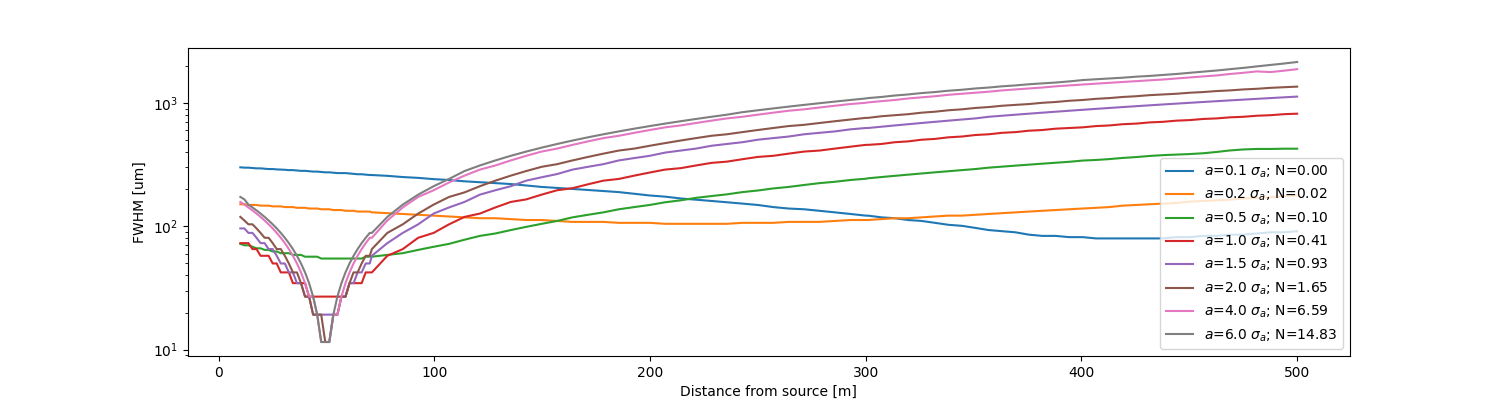
\includegraphics[width=0.95\textwidth]{figures/FigureG_1.png}
    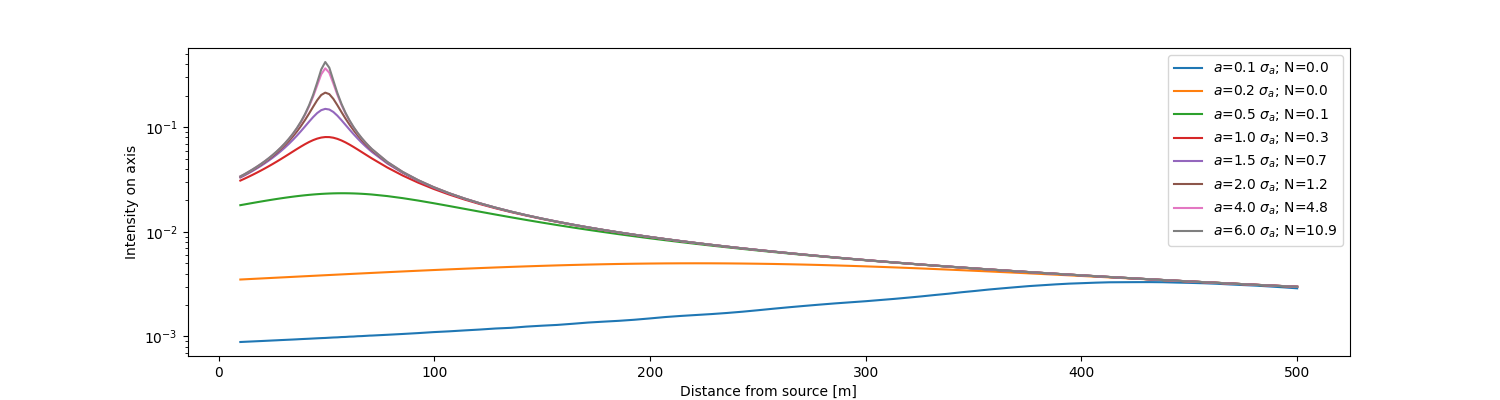
\includegraphics[width=0.95\textwidth]{figures/FigureG_2.png}
    \caption{Evolution of a beam cropped by a slit (modelled as a Gaussian window) and refracted by a lens as a function of the distance from the lens. a) evolution of the FWHM of the beam size, b) evolution of the intensity on-axis. The aperture is open at $a = n \sigma_a$ with $a=6,4,2,1.5,1,0.5,0.2,0.1$, $\sigma_a=$\SI{125}{\micro\meter}. The waist is found at a minumum of FWHM or a maximum of the intensity on-axis. The Fresnel number of the slit is also marked in the legend. }
    \label{fig:oneTFG}
\end{figure}

 
However, in real life the slit cannot be approximated by a Gaussian appodization window, but a rectangular-shaped function. This has important consequences: when the slit crops significantly the beam the Gaussian beam regime is broken therefore numerical calculation are necessary. Fig.~\ref{fig:oneTF} shows the beam evolution in this case.  It can be noticed that for $n=$6 or 4 ($N=$10.9,4.8, respectively) the situation does not change with respect to Fig.~\ref{fig:oneTFG} because the slit very sligtly crops the beam. For $n=2.0$ ($N=1.2$) the peak intensity at the waist reduces (although not changing position) and the evolution versus distance becomes wavy because the slit diffraction create new peaks in the beam intensity profile. 


NEXT IS TO INCLUDE REAL LENSES: NO EFFECT AS ONLY SINGLE Be LENS


NEXT IS PARTIAL COHERENCE


We now look at some relevant positions where some other beamline elements will be placed. These are positions $p_{fo1}=$\SI{164}{\meter} and   $p_{fo2}=$\SI{188}{\meter} measured from the source (\SI{99}{\meter} and \SI{123}{\meter} from the lens, respectively)
 
\begin{figure}
    \centering
    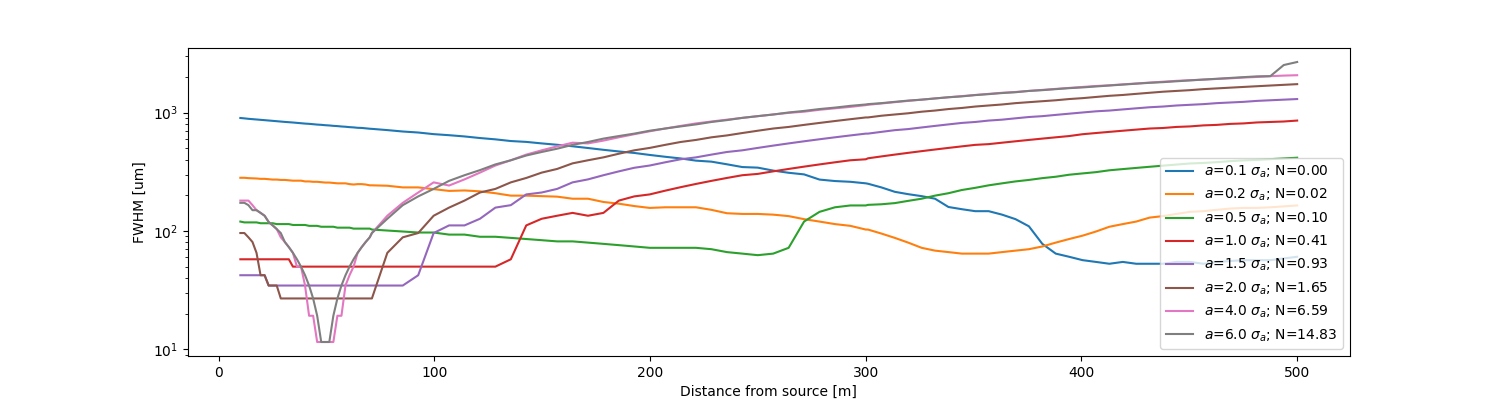
\includegraphics[width=0.95\textwidth]{figures/Figure_1.png}
    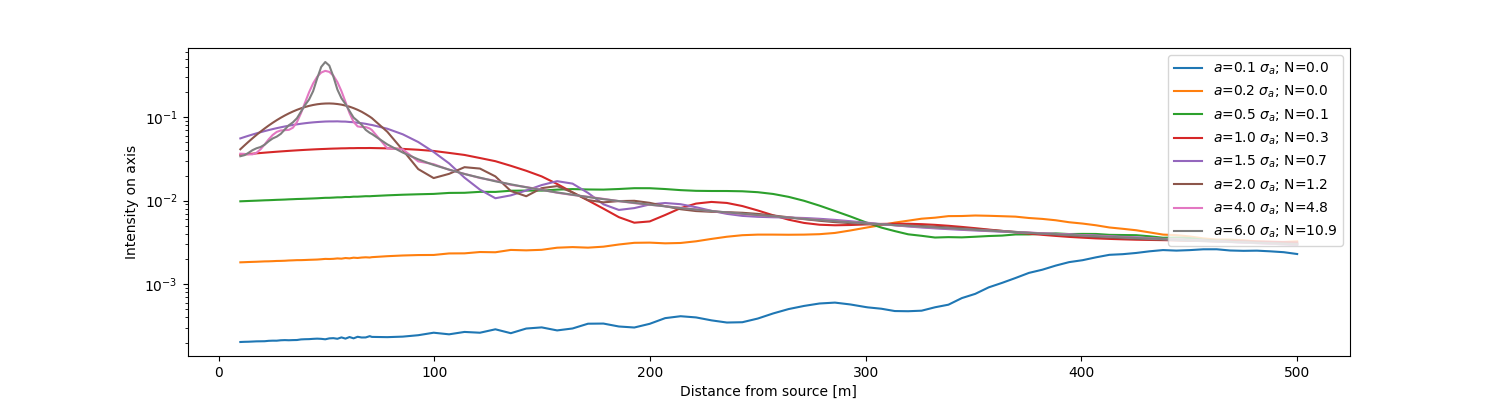
\includegraphics[width=0.95\textwidth]{figures/Figure_2.png}
    \caption{The same as in Fig.~\ref{fig:oneTFG} but the slit is modelled with a more realistic rectangular-shaped window.}
    \label{fig:oneTF}
\end{figure}

\section{Pairing transfocators}

Text text text text text text text text text text text text text text
text text text text text text text.

\section{A model for setting the transfocator configuration}

     % Appendices appear after the main body of the text. They are prefixed by
     % a single \appendix declaration, and are then structured just like the
     % body text.

\appendix
\section{Appendix title}

Text text text text text text text text text text text text text text
text text text text text text text.


     %-------------------------------------------------------------------------
     % The back matter of the paper - acknowledgements and references
     %-------------------------------------------------------------------------

     % Acknowledgements come after the appendices

\ack{Acknowledgements}

     % References are at the end of the document, between \begin{references}
     % and \end{references} tags. Each reference is in a \reference entry.

% \begin{references}
% \reference{Author, A. \& Author, B. (1984). \emph{Journal} \textbf{Vol}, 
% first page--last page.}
% \end{references}
\cite{knuth84}

%% Note added by Overleaf: If using bibtex, remove the "references" environment above, and uncomment the following lines.
\bibliographystyle{iucr}
\referencelist{iucr}

     %-------------------------------------------------------------------------
     % TABLES AND FIGURES SHOULD BE INSERTED AFTER THE MAIN BODY OF THE TEXT
     %-------------------------------------------------------------------------

     % Simple tables should use the tabular environment according to this
     % model

\begin{table}
\caption{Caption to table}
\begin{tabular}{llcr}      % Alignment for each cell: l=left, c=center, r=right
 HEADING    & FOR        & EACH       & COLUMN     \\
\hline
 entry      & entry      & entry      & entry      \\
 entry      & entry      & entry      & entry      \\
 entry      & entry      & entry      & entry      \\
\end{tabular}
\end{table}

     % Postscript figures can be included with multiple figure blocks

\begin{figure}
\caption{Caption describing figure.}
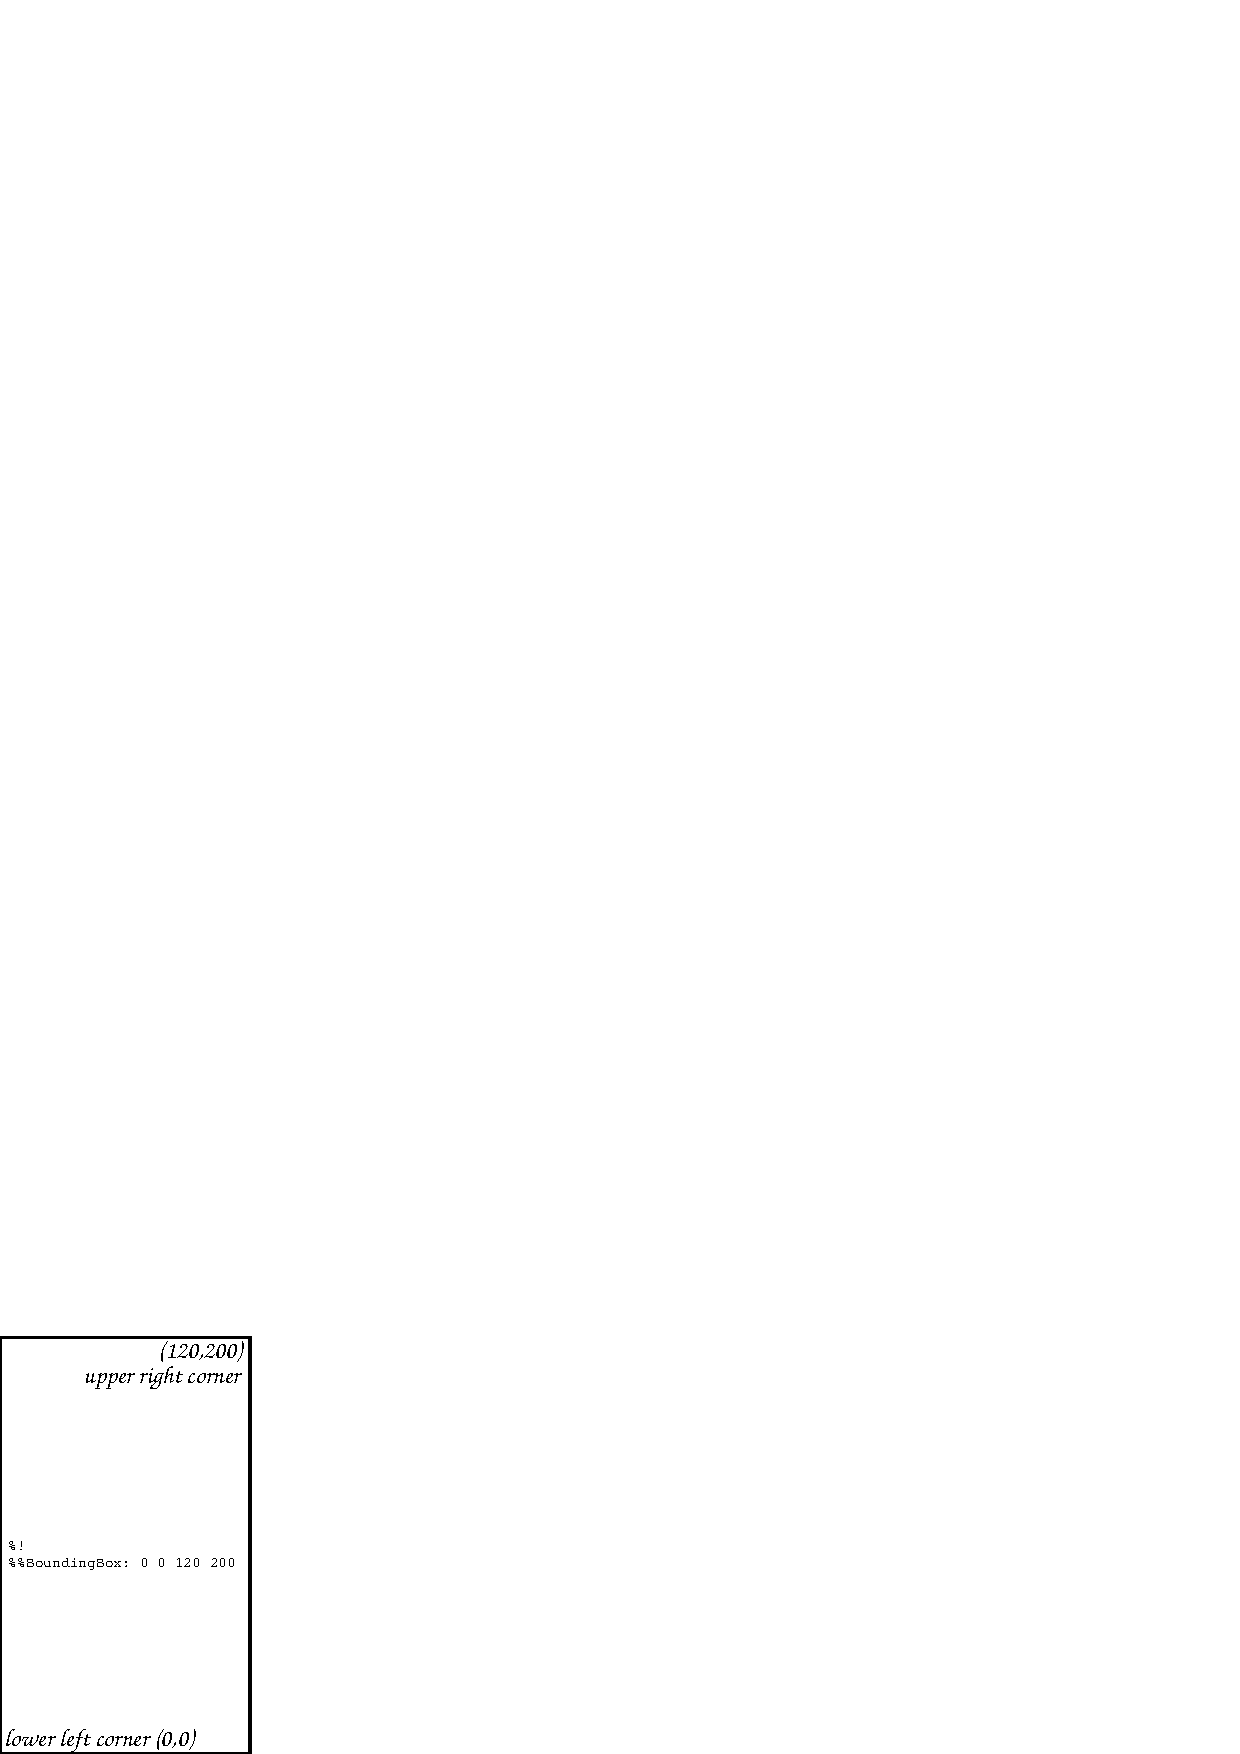
\includegraphics{fig1}
\end{figure}


\end{document}                    % DO NOT DELETE THIS LINE
%%%%%%%%%%%%%%%%%%%%%%%%%%%%%%%%%%%%%%%%%%%%%%%%%%%%%%%%%%%%%%%%%%%%%%%%%%%%%%
